% ex: ts=2 sw=2 sts=2 et filetype=tex
% SPDX-License-Identifier: CC-BY-SA-4.0
\begin{frame}
    \frametitle{Contenido}
    \tableofcontents
\end{frame}

\section{Elementos básicos de un programa}

\begin{frame}[c]{Elementos básicos de un programa}
  \begin{center}
    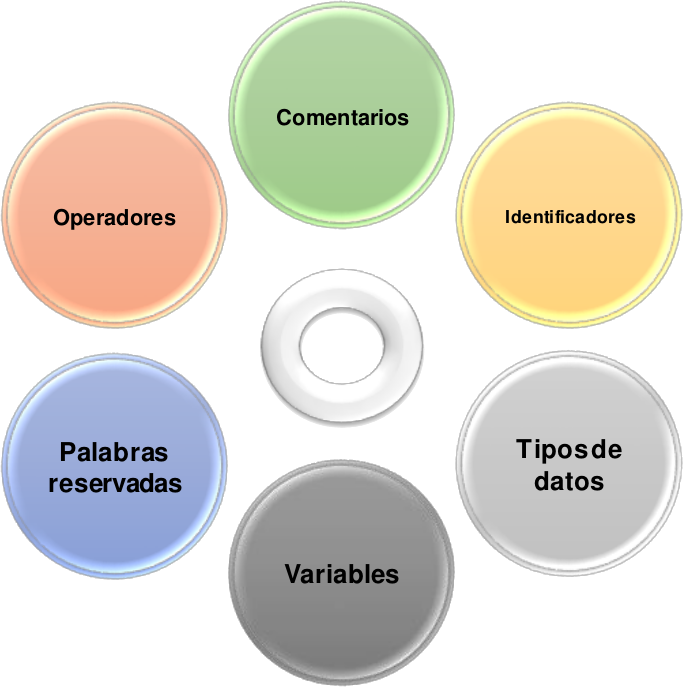
\includegraphics{020-elementos_basicos.png}
  \end{center}
\end{frame}

\begin{frame}[c]{Comentarios}
  \begin{itemize}
    \item Proporcionan una explicación en lenguaje humano de cómo
      funciona un algoritmo en particular, o una parte de él.
    \pausa
    \item Puede ser tan general o detallado como sea necesario.
    \pausa
    \item Es ignorado por el compilador (o intérprete).
    \pausa
    \item Se puede colocar en cualquier lugar del código fuente.
    \pausa
    \item Deben contener sólo información que sea relevante para la
      lectura y entendimiento del programa.
    \pausa
    \item Son esenciales en la fase de documentación.
    \pausa
    \item Cada lenguaje de programación define su propia sintaxis para los
      comentarios.
  \end{itemize}
\end{frame}

\begin{frame}[fragile]
  \frametitle{Comentarios}
  \begin{itemize}
    \item Los comentarios en \textbf{PSeInt} comienzan con los caracteres
      \textbf{//} y terminan hasta el fin del renglón.
  \end{itemize}
  \pausa
  Ejemplo:
  \begin{lstlisting}[style=pseudocodigo]
Algoritmo suma_de_dos_numeros
  // Ingresamos el primer número
  Escribir "Dame el primer número"
  Leer N1
  // Ingresamos el segundo número
  Escribir "Dame el segundo número"
  Leer N2
  // Hacemos la operación
  Suma <- N1 + N2
  // Mostramos el resultado
  Escribir "El resutlado es:", Suma
FinAlgoritmo
  \end{lstlisting}
\end{frame}

\begin{frame}[c]{Identificadores}
  \begin{itemize}
    \item Son los nombres de las unidades de programación definidas por el
      programador
      \begin{itemize}
        \item Variables, constantes
        \item Funciones, procedimientos, métodos, procesos
        \item Tipos de datos, clases, estructuras, arreglos
        \item Unidades, librerías, paquetes, programas
      \end{itemize}
    \pausa
    \item Un identificador puede contener letras, dígitos y ciertos caracteres
    %\item 
    %\item 
    %\item 
  \end{itemize}
\end{frame}
